\begin{theo}[Magnetische velden]{Magnetische velden}
    Net zoals we rondom een elektrische lading een elektrisch veld hebben gedefinieerd, kunnen we rond een magneet een magnetisch veld
    definiëren. Magnetische veldlijnen op tekeningen hebben dusdanig ook dezelfde eigenschappen als elektrische veldlijnen, namelijk

    \begin{minipage}{.7\textwidth}
        \begin{itemize}
            \item de richting van het magnetische veld is tangentieel met de magnetische veldlijnen
            \item de hoeveelheid magnetische veldlijnen per oppervlakte duidt op het sterkte van het magnetische veld
        \end{itemize}

    \end{minipage}
    \begin{minipage}{.24\textwidth}
        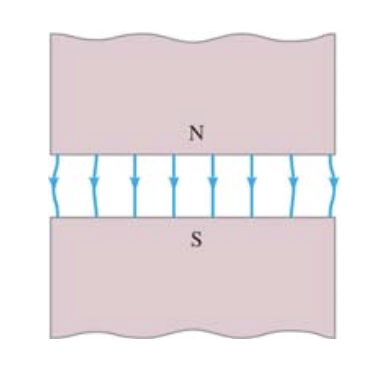
\includegraphics[scale = 0.5]{Images/Magnetisme/HomogeenMagnetischVeld}
    \end{minipage}

    \noindent De bijlage toont het triviale voorbeeld van een homogeen magnetisch veld.
\end{theo}

\begin{app}[Elekrtische stroom]{Elekrtische stroom}
    Elektrische stroom \textbf{produceert} een magnetisch veld. Een niet-magnetische, geleidende draad is dus wel magnetisch als we er stroom op zetten.
    Om de richting van het magnetisch veld te weten, kunnen we de \textbf{rechterhandregel} toepassen:

    \begin{minipage}{.8\textwidth}
        pak de draad vast met je rechterhand en steek je duim uit in
        de richting van de conventionele stroomzin en vouw je vingers dicht in de richting van het magnetische veld.
    \end{minipage}
    \begin{minipage}{.16\textwidth}
        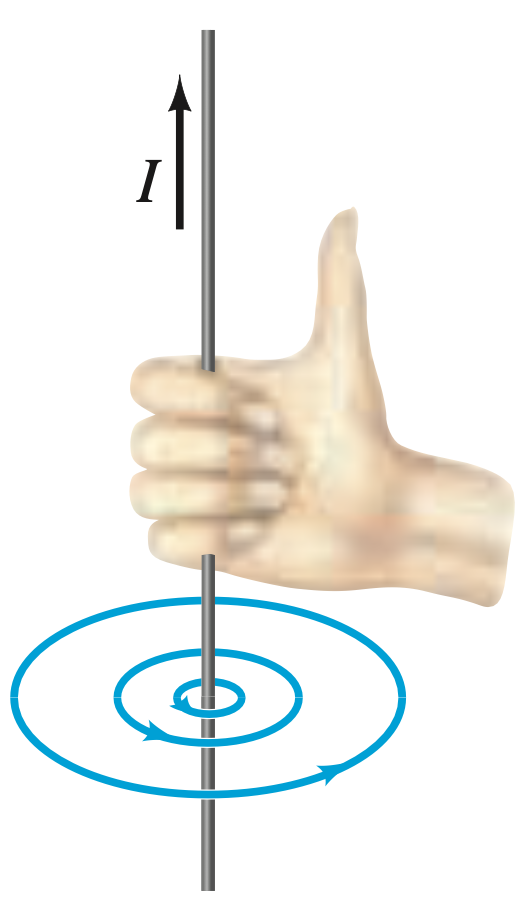
\includegraphics[scale = 0.2]{Images/Magnetisme/Rechterhandregel}
    \end{minipage}

\end{app}